\documentclass[12pt,fleqn]{article}\usepackage{../../common}
\begin{document}
Ders 27

Uclu entegralleri gorduk, pek cok kordinat sisteminde bu hesaplari
yapabiliyoruz. Simdi vektor alanlarini isleyecegiz, ozellikle akis (flux)
ve is (work) kavramlarina bakacagiz. 

Uzayda Vektor Alanlari

Vektor alani demek, her noktada bir vektor olmasi demek, bu vektorun
her ogesinin $x,y,z$ kordinatlarina bagli olmasi demek. Alan $\vec{F}$
icin mesela 

$$
\vec{F} = < P,Q,R >
$$

olabilir ve $P,Q,R$ birer fonksiyondur, $P(x,y,z)$ gibi. 

Ornekler

a)

Mesela kuvvet alanlari, yercekim kuvveti gibi, belli bir noktada belli
bir yone bir kuvvet etkisi var, bu bir kuvvet alani, vektor alani olarak
gosterilebilir. Yercekim alani orijin (0,0,0)'a dogru olan bir cekim kuvveti
olsun, ve buyuklugu $\frac{c}{\rho^2}$ gibi bir sabite oranli olsun, ki
$\rho$ orijine olan uzaklik. Kabaca bir resimde gosterirsek,

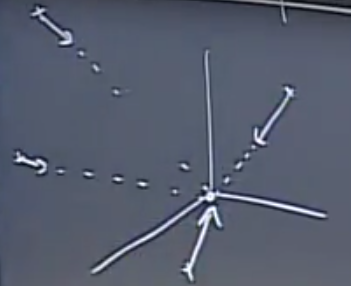
\includegraphics[width=20em]{calc_multi_27_01.png}

Goruldugu gibi cekim (ok) orijine dogru ve vektor buyuklugu (cekim kuvveti)
uzaklik arttikca kuculuyor. Birkac vektor cizdik sadece fikir vermesi
icin. Formulle belirtmek gerekirse,

$$
\vec{F} = \frac{-c < x,y,z >}{\rho^2}
$$

$< x,y,z >$'nin negatifi alindi, $< x,y,z >$ vektoru orijinden $x,y,z$'ye giden
vektor, oradan geri isaret eden vektor bunun negatif olurdu. Buyuklugu ise
$-c / \rho^2$ ile carparak ayarliyoruz. 

Benzer ornekler cogaltilabilir, elektrik alanlari, manyetik alanlar, vs.

b) 

Hiz alanlari bir diger ornek. Mesela sivi akisini temsil etmek istiyorsak,
ya da atmosferdeki ruzgar akisini incelemek istiyorsak, bunlari birer hiz alani
olarak gosterilebilir.

c)

Gradyan alanlari

Bir fonksiyon $u = u(x,y,z)$'nin gradyani $\nabla u = < u_x, u_y, u_z >$
bir gradyan alani olusturur.

Tabii ustteki ornekleri cok kesin hatlarla birbirinden ayri gibi gormemek lazim,
mesela elektrik ya da yercekim alanlari elektrik ya da yercekimsel potansiyel
fonksiyonunun gradyan alanidir. Gradyan matematiksel bir teknik, pek cok
yerde karsimiza cikabiliyor.

Yani vektor alanlari faydali seyler, bunu gorduk. Onlarla ne yapacagiz?
Akis konusu ile baslayalim.

Akis (Flux)

Daha once akis kavramini iki boyutta gormustuk,

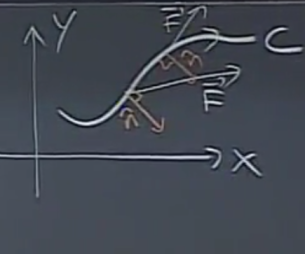
\includegraphics[width=10em]{calc_multi_27_02.png}

Bir vektor alani $\vec{F}$ icinde egri $C$ vardi, vektor alaninin
egriye dik olan bileseni ile bir akis entegrali olusturmustuk, bu
bir cizgi entegraliydi, formulu

$$
\int_C \vec{F} \cdot \hat{n} \ud s
$$

ki bu hesabin olctugu vektor alaninin ne kadar egri icinden, uzerinden
gectigiydi.  Sivi mekanigi icin mesela bu bir hiz alani uzerinden bize egri
uzerinden ne kadar sivi aktigini gosterebilirdi. Peki uc boyutta ne olur? Uc
boyutta tek egri uzerinden, mesela esen ruzgar hesabi biraz anlamsiz.
Bir yuzey uzerinden bu tur bir hesap daha anlamli.










[devam edecek]

\end{document}
